%--------------------------------------------------------------------------
%--------------------------------------------------------------------------
\section{Zero-inflated Poisson for species distribution} \label{sec:zip}
%--------------------------------------------------------------------------

%--------------------------------------------------------------------------
\subsection{Data and question}
%--------------------------------------------------------------------------
Species distribution models (SDM) aim at understanding how environmental conditions affect the abundance of a given species in a given site. The data are typically collected in the following way: $n$ sites are visited and in each site $i$ ($1 \leq i \leq n$) a $d$-dimensional vector $x_i$ of environmental descriptors is recorded, as well as the number $y_i$ of individuals of the species observed in the site.

\begin{figure}[ht]
  \begin{center}
    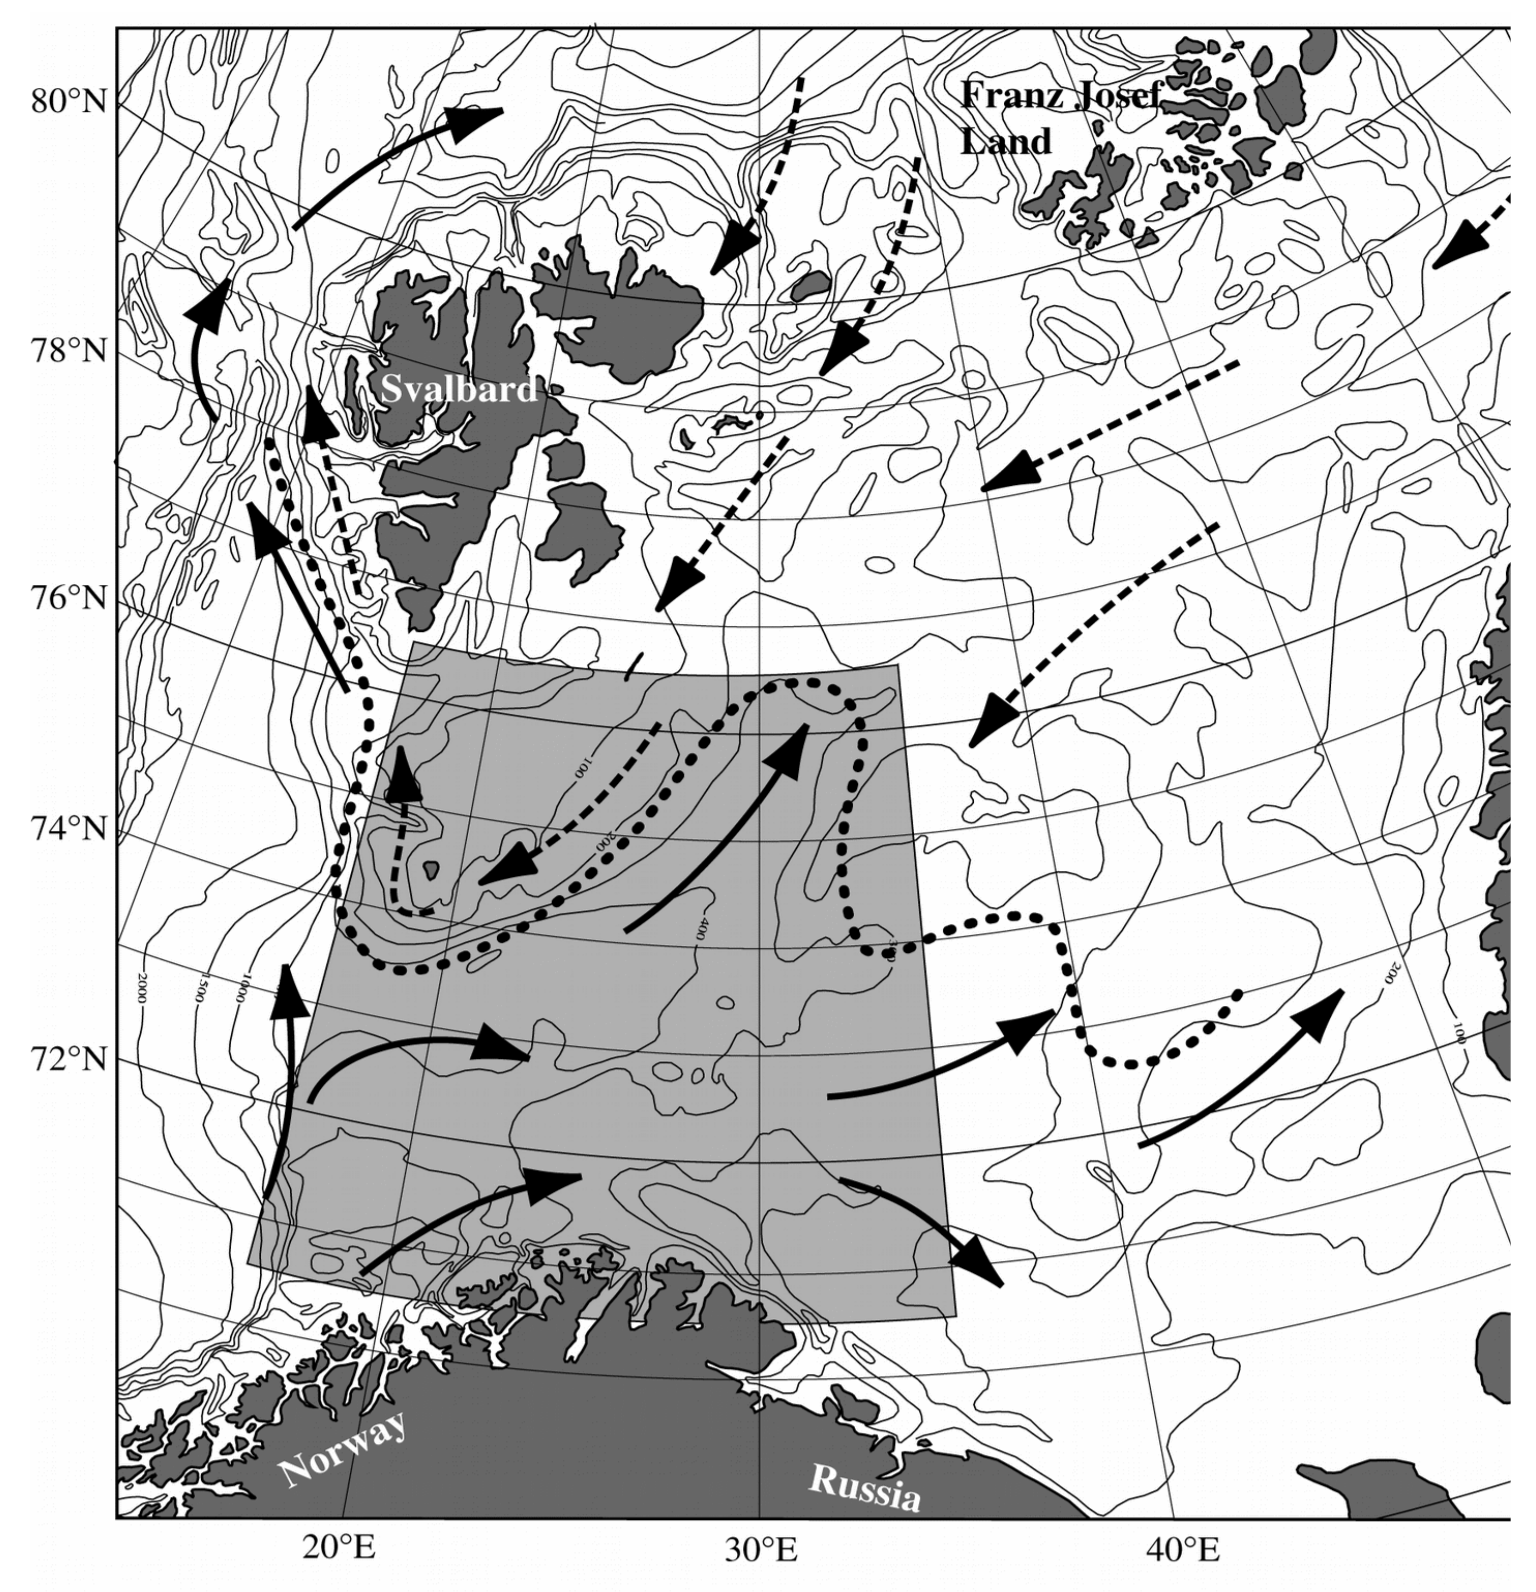
\includegraphics[width=.5\textwidth]{../Figures/BarentsFishMap}
    \caption{Map of the Barents sea, where data from Example \ref{ex:ZIPcodBarents} were collected. \label{fig:ZIPcodBarentsMap}}
  \end{center}
\end{figure}


\begin{dataset}[Cod in the Barents sea] \label{ex:ZIPcodBarents}
  \cite{fossheim2006fish} measured the abundance of cod ({\it Gadus morhua}) measured in $n=89$ stations of the Barents sea. In each station, fishes were captured according to the same protocole,  the latitude and longitude of each site were measured together with two environmental covariates: depth and temperature of the water. The data are available from the \url{PLNmodels} R package \citep{CMR21}. Figure \ref{fig:ZIPcodBarentsMap} gives a map of the Barents sea where the data were collected. Figure \ref{fig:ZIPcodBarentsData} gives the first few lines of the dataset and the histogram of the observed abundances, which display a large variance  and a high number of observations equal to $0$: the species is actually not observed (i.e. $y_i = 0$) in $n_0 = 61$ stations.
\end{dataset}

\begin{figure}[ht]
  \begin{center}
    \begin{tabular}{cc}
%         Data table & Histogram of abundances \\
      \begin{tabular}{l|rrrrr} 
        & Latit. & Longit. & Depth & Temp. & Abundance \\ 
        \hline 
        1 & 71.10 & 22.43 & 349 & 3.95 & 309 \\ 
        2 & 71.32 & 23.68 & 382 & 3.75 & 1041 \\ 
        3 & 71.60 & 24.90 & 294 & 3.45 & 218 \\ 
        4 & 71.27 & 25.88 & 304 & 3.65 & 77 \\ 
        5 & 71.52 & 28.12 & 384 & 3.35 & 13 \\ 
        6 & 71.48 & 29.10 & 344 & 3.65 & 196 
      \end{tabular}      
      &
      \begin{tabular}{c} 
        \includegraphics[width=0.4\textwidth, trim=0 15 10 0, clip=]{../Figures/CodBarents-Hist}
      \end{tabular}
    \end{tabular}
  \end{center}
  \caption{Cod abundance in the Barents sea. Left: head of the data table. Right: Histogram of the observed abundances. \label{fig:ZIPcodBarentsData}}
\end{figure}

--------------------------------------------------------------------------
\paragraph{Classical Poisson or logistic regression approaches.} 
The Poisson regression model (which is special instance of generalized linear models, see Appendix \ref{app:exponFamily}) provides a natural and well established framework for such count data.
This model states that the sites are all independent and that the mean number of observed individuals in site $i$ depends linearly on the covariates, through the log link function: 
\begin{equation} \label{eq:ZIPpoissonReg}
  \{Y_i\}_{1 \leq i \leq n} \text{ independent}, \qquad
  Y_i \sim \Pcal(\lambda_i), \qquad
  \log(\lambda_i) = x_i^\top \beta.
\end{equation}
The model can be adapted to account for heterogeneous sampling efforts (e.g. different observation times) by adding an known site-specific offset term $o_i$ to the regression model:
\begin{equation} \label{eq:ZIPpoissonRegOffset}
\log(\lambda_i) = o_i + x_i^\top \beta.
\end{equation}
The unknown parameter $\theta$ is only the vector of regression coefficients $\beta$, its estimation (by maximizing the likelihood) and interpretation are straightforward. \\
Still, this model suffers an important limitation because, if the species is actually absent from the site, the parameter $\lambda_i$ of the Poisson regression model should be zero (whatever the sampling effort), but Model \eqref{eq:ZIPpoissonReg} is not defined in this case. 

Alternatively, one may aim at understanding the drivers of the simple presence of the species in each site. 
One way is to consider the binary variable  $\widetilde{Y}_i = \Ind{Y_i >0}:$ 
$$
\widetilde{Y}_i = \left\{ 
\begin{array}{cll}
 1 & \mbox{ the species has been observed in site $i$}\\
 0 & \mbox{ otherwise, }
\end{array}
\right. 
$$
and to use a logistic regression model:
\begin{equation} \label{eq:ZIPlogisticReg}
  \{\widetilde{Y}_i\}_{1 \leq i \leq n} \text{ independent}, \qquad
  \widetilde{Y}_i \sim \Bern(\pi_i), \qquad
  \log\left(\frac{\pi_i}{1 - \pi_i}\right) = x_i^\top \alpha.
\end{equation}
This model also suffers limitation, because the presence of the species is not directly observed. Indeed, whenever the species is not observed ($Y_i = 0$), it is not possible to decide whether it is actually absent from the site, or simply unobserved (the two cases are sometimes referred to as 'true zero' versus 'false zero').

%--------------------------------------------------------------------------
\subsection{The ZIP model}
%--------------------------------------------------------------------------
A way to circumvent both limitations is to include in the model a variable $\lat_i$, that indicates whether the species is actually present or not:
$$
\lat_i = \left\{\begin{array}{ll}
              0 & \text{if the species is actually absent (and not only unobserved) in site $i$}\,, \\
              1 & \text{if the species is actually present (but possibly not observed) in site $i$}\,. 
            \end{array}\right.
$$
The variable $Z_i$ is obviously latent, because not observed. The distribution observed abundance $Y_i$ can then be defined conditionally on $Z_i$, yielding the zero-inflated Poisson (ZIP) model, which states that 
\begin{itemize}
  \item the sites are independent, 
  \item the binary variable $Z_i$ depends on the environment through a logistic regression model,
  \item if the species is absent ($Z_i = 0$), then the observed abundance $Y_i$ can only be zero, whereas if it is present, the observed abundance depends on the covariates through a Poisson regression model.
\end{itemize}
\begin{model}[Zero-inflated Poisson regression model] \label{mod:zip}
  \begin{align*} 
    \{(Y_i, Z_i)\}_{1 \leq i \leq n} & \text{ independent}, & 
    Z_i & \sim \Bcal(\pi_i), & 
    \logit(\pi_i) & := \log\left(\frac{\pi_i}{1 - \pi_i}\right) = x_i^\top \alpha, 
    \nonumber \\
    & & Y_i \mid Z_i = 0 & \sim \delta_0, \\
    & & Y_i \mid Z_i = 1 & \sim \Pcal(\lambda_i), & 
    \log(\lambda_i) &  = x_i^\top \beta \nonumber 
  \end{align*}
  where $\delta_0$ stands for the Dirac mass in zero: $Y \sim \delta_0 \; \Leftrightarrow \; \Proba{Y = 0} = 1$.
\end{model}

\remarks
\begin{itemize}
	\item Again, an offset term $o_i$ can be added to the Poisson regression to account for heterogeneous sampling efforts. 
	\item 
	Note that Model \eqref{def:zipDist} is sometimes parameterized in terms of absence probability, which amounts at replacing the presence probability $\pi_i$ with the absence probability $1 - \pi_i$ and the vector of regression coefficients $\alpha$ with $-\alpha$.
	\item The ZIP model is in fact a particular mixture model as defined in the previous section (Section \ref{def:mixtureDist}) where
	the first component of the mixture is a Dirac distribution at $0$, and the second component is a Poisson distribution with parameter $\lambda$. The weight is $\pi$  
\end{itemize}
The parameters of Model \eqref{mod:zip} are
$$
\parobs = \beta, \quad \quad  \parlat = \alpha, \quad \quad \theta=(\alpha,\beta)
$$
where $\alpha$ and $\beta$ are both vectors of regression coefficients: $\alpha$ encodes the effects of the environmental covariates on the presence probability $\pi_i$ while $\beta$ encodes the effects of the same covariates on the mean observed abundance $\lambda_i$ of the species, provided it is present in the site.

The marginal distribution of the observed abundance $Y_i$ can be obtained by deconditioning on $Z_i$ and turns out to be a zero-inflated distribution.





\begin{definition} \label{def:zipDist}
  The random variable $Y$ over $\Nbb$ has a zero-inflated distribution $ZIP(\pi, \lambda)$ iff
  \begin{equation}\label{eq:ZIPprob} 
    \Proba{Y = 0}= (1 - \pi) + \pi e^{-\lambda}, 
  \qquad \text{and, for } y \geq 1, \quad
  \Proba{Y = y} = \pi e^{-\lambda} \frac{\lambda^y}{y!}.        
 \end{equation}
\end{definition}
Formula \eqref{eq:ZIPprob} which can be reformulated into a unique formula:
\begin{equation}\label{eq:ZIPprob2}
 \mathbb{P}_{\text{ZIP}}(Y=y) =(1 - \pi) \Ind{\{0\}}(y) + \pi e^{-\lambda} \frac{\lambda^y}{y!}. 
\end{equation}
  

 


\begin{proposition} \label{prop:zipRegMArg}
  Under Model \eqref{mod:zip}, the marginal distribution of the observed abundance $Y_i$ is a zero-inflated Poisson $ZIP(\pi_i, \lambda_i)$.
\end{proposition}

\begin{proof}[Proposition \ref{prop:zipRegMArg}]
The observed abundance $Y_i$ is zero either if the species is absent (with probability $1 - \pi_i$) or if it is present (with probability $\pi_i$), but unseen (which occurs with probability $e^{-\lambda_i}$). Then, for the observed abundance to be $y_i \geq 1$, we need to the species to be present (with probability $\pi_i$) and the count to be $y_i$ (with probability $e^{-\lambda_i} {\lambda_i^{y_i}}/{y_i!}$).
\end{proof}

%--------------------------------------------------------------------------
\paragraph{Graphical model.}
% Figure \ref{fig:ZIPzipGM} displays the oriented graphical model associated with the joint distribution $p_\theta(Y, \Z)$ for Model \eqref{mod:zip}. According this model the couples $\{(Y_i, Z_i)\}_{1 \leq i \leq n}$ are all independent.
The graphical model associated with the joint distribution $p_\theta(\allY, \allZ)$ for Model \eqref{mod:zip} is the same as this of the mixture model, given in Figure \ref{fig:gmmGM}. According to this model the couples $\{(Y_i, Z_i)\}_{1 \leq i \leq n}$ are all independent. 

% \begin{figure}[ht]
%   \begin{center}
%     \input{TikZ/ZipGM}
%     \caption{Graphical representation of the mixture model \eqref{mod:zip}.\label{fig:ZIPzipGM}}
%   \end{center}
% \end{figure}

%--------------------------------------------------------------------------
\subsection{Marginal and complete log-likelihoods}
%--------------------------------------------------------------------------


We denote $\ally = \{y_i\}_{1 \leq i \leq n}$. Because the sites are independent, the marginal log-likelihood  is
%$$
%p_\theta(\y) = \sum_{i=1}^n \log\left((1 - \pi_i) \delta_0(y_i) + \pi_i \Pcal(y_i; \lambda_i)\right).
%$$
$$
\log p_\theta(\ally) = \sum_{i=1}^n \log\left((1 - \pi_i) \Ind{\{0\}}(y_i) + \pi_i e^{-\lambda_i} {\lambda_i^{y_i}}/{y_i!}\right).
$$ 

Denoting $\allZ = \{Z_i\}_{1 \leq i \leq n}$, the complete likelihood of Model \eqref{mod:zip} is
\begin{align} \label{eq:ZIPzipComplete}
  \log p_\theta(\ally, \allZ)
  & = \log p_\theta(\allZ) + \log p_\theta(\ally \mid \allZ) \nonumber \\
  & = \sum_{i=1}^n Z_i \log \pi_i + (1 - Z_i) \log(1- \pi_i) 
  + \sum_{i=1}^n Z_i \left(-\lambda_i + y_i \log \lambda_i - \log(y_i!)\right).
  \end{align}


\subsection{EM algorithm for the ZIP model}



\begin{algorithm}[EM for the ZIP model]\label{algo:ZIP} 
	Starting from  $\theta^{(0)}$, repeat until convergence:
	\begin{description}
		\item[E-step.]  For all $i=1, \dots,n$,  compute:
		\begin{equation} \label{eq:ZIPtau}
			\postprob{i}^{(h)}  = \Proba[\theta]{Z_i = 1 \mid Y_i =y_i}
			=  \frac{(1 - \pi^{(h)}_i)\Ind{y_i > 0} + \pi^{(h)}_i e^{-\lambda^{(h)}_i}}{(1-\pi^{(h)}_i) + \pi^{(h)}_i e^{-\lambda^{(h)}_i}} \,.
		\end{equation}
		\item[M-step.] 	Update the estimate of $\theta$ as
		\begin{align}\label{eq:updateZIP}
      \alpha^{(h+1)} 
      & = \argmax_\alpha   \sum_{i=1}^n \postprob[h]{i} \log \pi_i + (1 - \postprob[h]{i}) \log(1- \pi_i)  & 
      & \mbox{with} & \logit(\pi_i) & = x_i^\top \alpha \\
      \beta^{(h+1)} 
      & = \argmax_\beta \sum_{i=1}^N \postprob[h]{i} \left(-\lambda_i + y_i \log \lambda_i - \log(y_i!)\right)  &
      & \mbox{with} & \lambda_i & = \exp(x_i^\top \beta). \nonumber
    \end{align}
% 		\begin{equation}\label{eq:updateZIP}
%       \begin{array}{ccccccl}
%       \alpha^{(h+1)} &=& 	\argmax_\alpha   
%       \sum_{i=1}^n \postprob[h]{i} \log \pi_i + (1 - \postprob[h]{i}) \log(1- \pi_i)  &\mbox{ with }&   
%       \logit(\pi_i) &=& x_i^\top \alpha\\
%       \beta^{(h+1)} &=& 	\argmax_\beta \sum_{i=1}^N \postprob[h]{i} \left(-\lambda_i + y_i \log \lambda_i - \log(y_i!)\right)  &\mbox{ with }&    \lambda_i &=& \exp(x_i^\top \beta)
%       \end{array}
%     \end{equation}
\end{description}
	
\end{algorithm}
\remark 
In this model, the update of the parameters at the M-step is not explicit. However, having a look at the quantities they have to maximise, we observe that they  have the same form as the log-likelihood of a classical logistic regression ($\widetilde{Y}_i$ being replaced with $\postprob[h]{i}$) for $\alpha$  and of a Poisson regression (with weights $\postprob[h]{i}$) for $\beta$. The optimization with respect to $\alpha$ and $\beta$ can be achieved numerically with standard libraries dedicated to generalized linear models.

\begin{proof}[Algorithm \ref{algo:ZIP}]

\paragraph{About $Q(\theta \mid \curpar)$.}
From the expression of the complete log-likelihood provided in Equation \eqref{eq:ZIPzipComplete}, the integration of the latent variables $Z_i$ leads to the following formula for $Q(\theta \mid \curpar)$: 
\begin{equation}\label{eq:ZIPQ}
Q(\theta \mid \theta^{(h)})
= \sum_{i=1}^n \postprob[h]{i} \log \pi_i + (1 - \postprob[h]{i}) \log(1- \pi_i) 
+\sum_{i=1}^n \postprob[h]{i} \left(-\lambda_i + y_i \log \lambda_i - \log(y_i!)\right),
\end{equation}
where 
$\postprob{i}^{(h)} = \Esp_{\curpar}[Z_i \mid \allYy=\ally]$. 


\paragraph{E-step.}
To evaluate $Q(\theta \mid \curpar)$, we only need to evaluate the conditional expectation of each $Z_i$ given the data $\ally$, that is to evaluate $\postprob{i}^{(h)} = \Esp_{\curpar}[Z_i \mid \allYy=\ally]$. This can be done in closed form. \\
First, observe that, because the couples $(Y_i, Z_i)$ are all independent from each other, the conditional distribution of $Z_i$ given $\allY$ is the same as its conditional distribution given the corresponding  $Y_i$ only: $
\postprob{i}^{(h)} = \Esp_{\curpar}[Z_i \mid Y_i=y_i]$. 
Furthermore, because the $Z_i$ are 0/1, we know that $$ \postprob{i}^{(h)} = \Esp_{\curpar}[Z_i \mid Y_i=y_i] = \Proba[\curpar]{Z_i = 1 \mid Y_i=y_i}.$$ \\
From Model \eqref{mod:zip}, we easily see that if the observed count is not zero ($y_i > 0$), then the species is surely present, so 
\begin{equation}\label{eq:ZIPtau1}
\Proba[\curpar]{Z_i = 1 \mid Y_i >0} = 1.
\end{equation}
If the observed count is $y_i=0$, we can apply the Bayes formula: 
\begin{eqnarray}\label{eq:ZIPtau2}
\Proba[\curpar]{Z_i = 1 \mid Y_i= 0} &=&  \frac{\Proba[\curpar]{Y_i= 0 ,  Z_i = 1}}{\Proba[\curpar]{Y_i= 0}} = \frac{\Proba[\curpar]{Y_i= 0 \mid   Z_i = 1}\Proba[\curpar]{Z_i=1}}{\Proba[\curpar]{Y_i= 0 }}\nonumber\\
 &=& \frac{\pi^{(h)}_i e^{-\lambda^{(h)}_i}}{ (1-\pi^{(h)}_i) + \pi^{(h)}_i e^{-\lambda^{(h)}_i}}  \quad \mbox{(using Equation \eqref{eq:ZIPprob2} with $y_i=0$)}
\end{eqnarray}
Now, combining Equations \eqref{eq:ZIPtau1} and \eqref{eq:ZIPtau2}, we obtain a global formula: 
\begin{equation*} %\label{eq:ZIPtau}
\postprob{i}^{(h)}: =\tau(y_i) = \Esp_{\curpar}[Z_i \mid Y_i=y_i] 
=  \Ind{y_i > 0} + \frac{\pi^{(h)}_i e^{-\lambda^{(h)}_i}}{(1-\pi^{(h)}_i) + \pi^{(h)}_i e^{-\lambda^{(h)}_i}} \Ind{y_i = 0}
=\frac{(1 - \pi^{(h)}_i)\Ind{y_i > 0} + \pi^{(h)}_i e^{-\lambda^{(h)}_i}}{(1-\pi^{(h)}_i) + \pi^{(h)}_i e^{-\lambda^{(h)}_i}} \,.
\end{equation*}
%\PGcom{J'ai réécrit la formule complète avec les indicatrices}
%\SRcom{J'ai utiliser l'autre forme des indicatrices : il faudra trancher}
%\begin{equation} \label{eq:ZIPtau}
%\postprob{i} = \frac{\pi_i e^{-\lambda_i}}{(1-\pi_i) + \pi_i e^{-\lambda_i}}.
%\end{equation}


%--------------------------------------------------------------------------
\paragraph{M step.}
We may now update the parameter $\theta$ by maximizing the objective function of the EM algorithm provided in Equation \eqref{eq:ZIPQ}. %, 
Reminding that $$\pi_i = \exp(x_i^\top \alpha) /(1 + \exp(x_i^\top \alpha)) \quad \mbox{ and } \quad  \lambda_i = \exp(x_i^\top \beta),$$ we observe that $Q(\theta \mid \theta^{(h)})$ can be decomposed into a sum of two terms depending respectively in $\alpha$ and $\beta$: 
\begin{eqnarray*}	
A^{(h)}(\alpha) &=& \sum_{i=1}^n \postprob[h]{i} \log \pi_i + (1 - \postprob[h]{i}) \log(1- \pi_i) \\
B^{(h)}(\beta)&=& \sum_{i=1}^n \postprob[h]{i} \left(-\lambda_i + y_i \log \lambda_i - \log(y_i!)\right) 
\end{eqnarray*}
which can be optimized separately: 
$$
\argmax_\alpha Q(\theta \mid \theta^{(h)}) = \argmax_\alpha A^{(h)}(\alpha)
\qquad \text{and} \qquad 
\argmax_\beta Q(\theta \mid \theta^{(h)}) = \argmax_\beta B^{(h)}(\beta).
$$

\end{proof}
%--------------------------------------------------------------------------
\subsection{Illustration}
%--------------------------------------------------------------------------
We now compare the ZIP regression \eqref{mod:zip} with the logistic regression \eqref{eq:ZIPlogisticReg} and Poisson regression \eqref{eq:ZIPpoissonReg} on the cod abundances introduced in Dataset \ref{ex:ZIPcodBarents}. To ease the interpretation and the comparison of the regression coefficients, the four covariates were centered and their variances were set to one. Models \eqref{eq:ZIPlogisticReg} and \eqref{eq:ZIPpoissonReg} can be fitted with the R {\tt glm} R function, and model \eqref{mod:zip} with the {\tt zeroinfl} function of the {\tt pscl} R package.

%--------------------------------------------------------------------------
\paragraph{Parameter estimates.}
Table \ref{tab:codBarentsCoefs} gives the MLE of the regression coefficients for the Poisson regression , the logistic regression  and the ZIP regression \eqref{mod:zip} models. We observe that the regression coefficients for both the presence probability ($\alpha$) and the abundance ($\beta$) are different when dealing with both aspect separately (i.e logistic regression or Poisson regression) or jointly (ZIP regression). 
As the covariates have been centered, one may focus on the intercepts, which control the presence probability and the abundance, respectively, in a 'mean' site. 
% \PGcom{C'est plutôt l'abondance et la proba de présence sur un site "moyen", il me semble} 
% \SRcom{Quelle est la différence littérale ?}
The ZIP regression yields a higher mean presence probability than the logistic, because it accounts for the fact that the species can be present, when it is actually not observed. 
% \PGcom{L'intercept est plus faible pour le ZIP. Je ne sais pas si l'interprétation est si claire. Pour moi, je lis que, pour le site "moyen" (qui n'existe peut être pas), le ZIP prévoit qu'il y a moins de chance d'en voir que le modèle logistique.} 
% \SRcom{Corrigé : il y a avait une erreur dans le report des signes.}
As for the Poisson part (which deals with the mean abundance), the Poisson regression yields a smaller mean abundance, as it needs to accommodate for the numerous zeros in the data set, whereas the abundance part of the ZIP regression only deals with case where the species is actually present.

\begin{table}[ht]
  \begin{center}
    \begin{tabular}{l|rrrrr|rrrrr} 
      & \multicolumn{5}{c|}{Presence ($\alpha$)} & \multicolumn{5}{c}{Abundance ($\beta$)} \\
      & Inter. & Lat. & Long. & Depth & Temp. & Inter. & Lat. & Long. & Depth & Temp. \\
      \hline
      Logistic \eqref{eq:ZIPlogisticReg} & -1.275 & -0.251 & 0.301 & -0.387 & 1.994 & -- & -- & -- & -- & -- \\ 
      Poisson \eqref{eq:ZIPpoissonReg} & -- & -- & -- & -- & -- & 0.010 & -0.721 & -0.043 & 0.917 & 2.479 \\ 
      ZIP \eqref{mod:zip} & -0.95 & -0.287 & 0.374 & -0.578 & 1.59 & 1.543 & -0.371 & -0.265 & 0.864 & 1.858 
    \end{tabular} 
    \caption{Cod abundance in the Barents sea.  \label{tab:codBarentsCoefs}}
  \end{center}
\end{table}

%--------------------------------------------------------------------------
\paragraph{Presence probability.}
Figure \ref{fig:ZIPcodBarentsFit-presence} (left) gives the estimated probability $\widehat{\pi}_i^{ZIP}$ of presence in each station for Example \ref{ex:ZIPcodBarents}, as a function of the linear predictor $x_i^\top \widehat{\alpha}^{ZIP}$. The blue crosses indicate the probability of presence according to the logistic regression $\pi_i^{logistic}$: we see that the two models yield similar probabilities. Still, the binary part of the ZIP model (encoded in $\pi_i^{ZIP}$) does not contain all information, regarding the prediction of the actual presence of the species in a given site: the abundance part must also be accounted for.

Indeed, under the ZIP model \eqref{mod:zip}, the sites can classified in term of actual presence or absence of the species of species, using the same rule as this used to classify observations into components under a mixture model, as seen in Section \ref{sec:gmm}. This ZIP classification is based on the estimate of the conditional probability $\postprob{i}$, given in Equation \eqref{eq:ZIPtau}. The right panel of Figure \ref{fig:ZIPcodBarentsFit-presence} compares the conditional probability $\postprob{i}^{ZIP}$ resulting from the ZIP model, with the presence probability $\pi_i^{logistic}$. We observed the classification based on $\postprob{i}^{ZIP}$ is much more contrasted than this based on $\pi_i^{logistic}$, which predicts very low probabilities of presence in sites where the species has actually been observed. This difference is greatly do the the fact that the logistic regression relies on degraded data, that is the $\widetilde{Y}_i$, instead of the observed counts $Y_i$.

\begin{figure}[ht]
  \begin{center}
    \begin{tabular}{cc}
      observed vs $\pi^{ZIP}$ (and $\pi^{logistic}$) &
      $\pi^{logistic}$ vs $\postprob{}^{ZIP}$ \\
      \includegraphics[width=0.3\textwidth, trim=0 15 10 30, clip=]{../Figures/CodBarents-PresProb-ZIP_Logistic} &
      \includegraphics[width=0.3\textwidth, trim=0 15 10 30, clip=]{../Figures/CodBarents-PresPred-ZIP-Logistic} 
    \end{tabular}
    \caption{Cod abundance in the Barents sea. % \\
    Left: probability of presence according to the ZIP model ($\widehat{\pi}_i^{ZIP}$: black curve), 
    dots = observed presence (black dots ($\bullet$): $Y_i > 0$, red dots (\textcolor{red}{$\bullet$}): $Y_i = 0$), 
    blue crosses (\textcolor{blue}{$+$}): probability of presence according to logistic regression $\pi_i^{logistic}$. \\
    Right: prediction of presence according to the ZIP model ($x$ axis) vs prediction of presence according to the logistic regression ($y$ axis). Blue dotted lines = 50\% thresholds.
    \label{fig:ZIPcodBarentsFit-presence}}  
    \end{center}
\end{figure}

%--------------------------------------------------------------------------
\paragraph{Abundance prediction.}
Figure \ref{fig:ZIPcodBarentsFit} displays the fit of the Poisson regression model (left) and of the ZIP model (center): obviously, the variability of the data does not fit the expected variability under the simple Poisson assumption. The prediction intervals of the ZIP model better accounts for the additional variability due to the excess of zeros, but are much larger. \\
%\PGcom{Sur la figure de droite, l'intervalle de confiance fait un truc bizarre, non?}
The predictions provided by the ZIP regression model must be carefully analysed as they combine estimates of both the presence probability $\pi_i$ of the species in site $i$, and of its expected abundance $\lambda_i$ {\sl conditional on its presence}. Because the regression parameters are different for the two parameters, a high expected abundance $\lambda_i$ may coincide with a low presence probability $\pi_i$, as shown in the right panel of Figure \ref{fig:ZIPcodBarentsFit}. This explains the apparently erratic behavior of the prediction interval displayed in the center panel of Figure \ref{fig:ZIPcodBarentsFit}. 

\begin{figure}[ht]
  \begin{center}
    \begin{tabular}{ccc}
      observed vs Poisson($\beta$) &
      observed vs ZIP($\alpha, \beta$) & 
      $\widehat{\pi}^{ZIP}$ vs $\widehat{\lambda}^{ZIP}$ \\
      \includegraphics[width=0.3\textwidth, trim=0 15 10 30, clip=]{../Figures/CodBarents-Abundance-Poisson} &
      \includegraphics[width=0.3\textwidth, trim=0 15 10 30, clip=]{../Figures/CodBarents-Abundance-ZIP} &
      \includegraphics[width=0.3\textwidth, trim=0 15 10 30, clip=]{../Figures/CodBarents-Presence-Abundance-ZIP} 
    \end{tabular}
    \caption{Cod abundance in the Barents sea. % \\
    Left: observed abundances vs predicted abundances (in log-scale) with the Poisson regression \eqref{eq:ZIPpoissonReg}, dotted red lines $= 95\%$ interval for the Poisson distribution (\SR{}{1 is added to abundances to allow log-scale}). % \\
    Center: observed abundances vs predicted abundances  $\widehat{\lambda}_i$ (in log-scale) with the ZIP regression \eqref{mod:zip}, dotted red lines $= 95\%$ interval for the ZIP distribution. % \\
    Right: presence probability $\widehat{\pi}_i$ and expected abundance $\widehat{\lambda}_i$ estimated with the ZIP regression \eqref{mod:zip}. Red dots = sites where the species was not observed.
    \label{fig:ZIPcodBarentsFit}}
  \end{center}
\end{figure}

%--------------------------------------------------------------------------
\paragraph{Model comparison.}
We may compare the ZIP model with the Poisson regression, as they both deal with the observed counts $Y_i$, (whereas the logistic regression deals with the $\widetilde{Y}_i$). Their respective log-likelihood are
\begin{align*}
  \log p_{\widehat{\alpha}}^{Poisson}(\y) & = -1142.8 & & (\text{with $p=5$ independent parameters}), \\
  \log p_{\widehat{\alpha}, \widehat{\beta}}^{ZIP}(\y) & = -892.2 & & (\text{with $2 p=10$ independent parameters}).  
\end{align*}
% Because Model \eqref{eq:ZIPpoissonReg} is nested in Model \eqref{mod:zip}, the two models can be compared either with a log-likelihood ratio test (LRT) \PGcom{Il n'y a pas un problème théorique dû au fait que le modèle nul correspond à $\pi = 1$, qui est au bord du domaine?} or using the AIC or BIC criterion. 
% For the LRT, we obtain 
% $$
% LRT = 2 \left(\log p_{\widehat{\alpha}, \widehat{\beta}}^{ZIP}(\y) - \log p_{\widehat{\alpha}}^{Poisson}(\y)\right) = 501.3
% $$ 
% for $p = 5$ degrees of freedom (yielding a $p$-values below $10^{-100}$). 
Models \eqref{eq:ZIPpoissonReg} and \eqref{mod:zip} can be compared with AIC or BIC:
\begin{align*}
  AIC(Poisson) & = -1148, & AIC(ZIP) & = -902.2 \\
  BIC(Poisson) & = -1154, & BIC(ZIP) & = -914.6. 
\end{align*}
Both criteria concur to conclude to a much better fit of the ZIP regression model.
% \begin{tabular}{l|rrr} 
% model & nb parms & logL & BIC \\ 
% \hline 
% Poisson & 5 & -1142.8 & -1154 \\ 
% ZIP & 10 & -892.2 & -914.6 
% \end{tabular} 
%--------------------------------------------------------------------------
\subsection{Using the Louis' formula to get the asymptotic variance}\label{sec:AsympVarZIP}
%--------------------------------------------------------------------------
To conclude this section, we use the zero-inflated Poisson Model \ref{mod:zip} to illustrate the use of the Louis's formula \citep{Louis82} introduced in Section \ref{sec:asympVarMLE} to estimate the asymptotic variance of the MLE $\widehat{\theta}$. 
To make the calculations lighter, we consider a model \emph{with no covariates}, that is where, for all $1 \leq i \leq n$: $$\pi_i = \pi, \quad \lambda_i = \lambda, \quad \mbox{ and } \theta = (\pi, \lambda)$$





\begin{proposition}\label{prop:AsympVarZIP}
 
  For the ZIP model without covariates, let us define: 
  
  $$\allP = \sum_{i=1}^n \Ind{y_i > 0},  \quad \allY_+ = \sum_{i=1}^n y_i$$ and 
  $$ 
   \gamma = \frac{1}{\pi(1-\pi)},\quad   \eta = \frac{\pi e^{-\lambda}}{(1-\pi) + \pi e^{-\lambda}}, \quad  \quad V = (1-\eta)\eta (n-\allP). $$ 
  Then we have: 
  
  $$\mathbf{J}_\theta  S_\theta(\ally) =  \left(
  \begin{array}{cc}
  -\frac{\allP + (n-\allP) \eta}{\pi^2} - \frac{(n-\allP)(1 - \eta)}{(1 - \pi)^2} & 0 \\
  0 & - \frac{\allY_+}{\lambda^2}
  \end{array}
  \right) 
  + V  \left(
  \begin{array}{cc}
  \gamma^2  & -\gamma    \\
  -\gamma  & 1 
  \end{array}
  \right)$$
  
\end{proposition}

\begin{proof}[Proposition \ref{prop:AsympVarZIP}]
The proof is composed of three steps: first we calculate the derivatives of the complete likelihood, then we compute their conditional expectation given the observed data, and, finally, we gather all these results into the estimated Fisher information matrix.
\begin{description}

  \item[Complete log-likelihood] In absence of covariate, the complete likelihood \eqref{eq:ZIPzipComplete}  becomes
  \begin{align*}
    \log p_\theta(\ally, \allZ) 
    & = \sum_{i=1}^n Z_i \log \pi  + (1 - Z_i) \log(1- \pi ) 
    + \sum_{i=1}^n Z_i \left(-\lambda  + y_i \log \lambda  - \log(y_i!)\right)\\
    & = Z_+ \log \pi + (n- Z_+) \log(1 - \pi) - \allZ_ +\lambda + y_+ \log \lambda - L
  \end{align*}
  where 
  $$
  \allZ_+ = \sum_{i=1}^n Z_i,  
  \qquad  \allY_+ = \sum_{i=1}^n Z_i y_i =  \sum_{i=1}^n y_i 
  \qquad \mbox{and} \qquad L = \sum_{i=1}^n Z_i \log(y_i!) = \sum_{i=1}^n  \log(y_i!).
  $$
  The expressions $\allY_+$ and $L$ derive from the fact that $Z_i\in\{0,1\}$ and when $Z_i=0$,  $y_i=0$ so $y_i = y_iZ_i$. The same holds for $\log(y_i!)$. \\
 
  \item[Derivatives of the complete log-likelihood.]
   From this expression of the complete likelihood, we get the derivatives
  $$
  \partial_\pi \log p_\theta(\ally, \allZ) 
  = \frac{\allZ_+}{\pi} - \frac{n- Z_+}{1 - \pi}   =  \frac{1}{\pi(1-\pi)} \allZ_+ - \frac{n}{1 - \pi}\\
  =  \gamma \allZ_+ - \frac{n}{1 - \pi}
  $$
  where $\gamma = 1/\pi(1-\pi)$. 
  Besides, 
  $$
  \partial_\lambda \log p_\theta(\ally, \allZ) = - \allZ_+ + \frac{y_+}{\lambda},
  $$
  The Hessian is then obtained by calculating the second derivatives:
  \begin{equation}\label{eq:HessZIP}
    \partial^2_{\pi^2} \log p_\theta(\ally, \allZ) = - \frac{\allZ_+}{\pi^2} - \frac{n- \allZ_+}{(1 - \pi)^2}, 
    \qquad
    \partial^2_{\pi\lambda} \log p_\theta(\ally, \allZ) = 0, 
    \qquad
    \partial_{\lambda^2} \log p_\theta(\ally, \allZ) = - \frac{\allY_+}{\lambda^2}.
    \end{equation}
  %
  \item[Integration of the latent variables.]
  Louis' formulas then require to evaluate the conditional expectation of the Hessian matrix and the conditional variance of the gradient vector. A quick look at their formula enables us to conclude that we need to compute the conditional expectation and variance of $Z_+ = \sum_{i=1}^n Z_i$, that is
  $$
  \Esp[ \allZ_+ \mid \allYy]  
  = \sum_{i=1}^n \Esp[ Z_i \mid   \ally]= \sum_{i=1}^n \Esp[ Z_i \mid   Y_i=y_i] = \sum_{i=1}^n \tau(y_i)
  $$
  Denoting by $\eta$ the probability for the species to be present given that $Y_i=0$
  $$
  \eta = \frac{\pi e^{-\lambda}}{(1-\pi) + \pi e^{-\lambda}},
  $$
  we have from Equation \eqref{eq:ZIPtau} that $\tau(y_i) = (1-\eta) \Ind{y_i > 0} + \eta$, so
  $$
  \Esp[ \allZ_+ \mid \allYy]  
  = \sum_{i=1}^n  (1-\eta) \Ind{y_i > 0} +  \eta =  (1-\eta) \allP  + n \eta
  = \allP + (n - \allP) \eta,
  $$
  where $\allP$ stands for the number of sites where the species is observed: $\allP = \sum_{i=1}^n \Ind{y_i > 0}$. \\
  Let us now consider the variance: by conditional independance of the $Z_i \mid \allYy$, we have that
  $$
  \Var[ \allZ_+ \mid \allYy]  = \sum_{i=1}^n \Var[ Z_i \mid   Y_i=y_i].
  $$ 
  Besides, we have demonstrated that $Z_i \mid \allYy$ is distributed as a Bernoulli with parameter $\tau_i = \tau(y_i)$ provided in Equation \eqref{eq:ZIPtau}, so 
  So 
  \begin{align*}
  \Var[ Z_i \mid \allYy] 
  &=  \tau_i (1- \tau_i)=  \left((1-\eta)\Ind{y_i>0} +\eta\right)(1-(1-\eta)\Ind{y_i>0} -\eta)\\
  &=  \left((1-\eta)\Ind{y_i>0} +\eta\right)(1-\eta)(1-\Ind{y_i>0})\\
  &= (1-\eta)[(1-\eta)\underbrace{\Ind{y_i>0}(1-\Ind{y_i>0})}_{=0}+\eta(1-\Ind{y_i>0})]\\
  &= (1-\eta)\eta (1-\Ind{y_i>0}),
  \end{align*}
  that is :
  $$
  \Var[ \allZ_+ \mid \allYy] = \sum_{i=1}^n (1-\eta)\eta (1-\Ind{y_i>0}) = (1-\eta)\eta (n-P).
  $$ 
  %
  \item[Expression of $\widehat{I}(\theta)$.]
  By injecting the expectation and variance of $Z_+$ into the Hessian  and the gradient, we can now derive the required conditional moments, that is
  \begin{align*}
      \Esp[\partial^2_{\pi^2} \log p_\theta(\ally, \allZ)\mid \allYy] 
      & = -\frac{P + (n-P) \eta}{\pi^2} - \frac{(n-P)(1 - \eta)}{(1 - \pi)^2}, &
      \Esp[\partial^2_{\pi\lambda} \log p_\theta(\ally, \allZ)\mid \allYy] 
      & = 0, \\
      \Esp[\partial_{\lambda^2} \log p_\theta(\ally, \allZ)\mid \allYy]
      & = - \frac{y_+}{\lambda^2}
  \end{align*}
  and
  \begin{align*}
      \Var[\partial_{\pi} \log p_\theta(\ally, \allZ)\mid \allYy]
      & = \gamma^2 \Var[Z_+\mid \allYy], \\
  %    = \gamma^2 (n - P) \eta (1 - \eta), \\
      \Var[\partial_{\lambda} \log p_\theta(\ally, \allZ)\mid \allYy]
      & = \Var[Z_+\mid \allYy], \\
  %    = \lambda^2 (n - P) \eta (1 - \eta) \\
      \Cov[\partial_{\pi} \log p_\theta(\ally, \allZ), \partial_{\lambda} \log p_\theta(\ally, \allZ)\mid \allYy]
      & = - \gamma \Var[Z_+\mid \allYy],% &
  %    \SR{}{\text{where} \quad \Var[Z_+\mid \allYy]} & \SR{}{= \sum_{i=1}^n \Var[Z_i \mid Y_i]}
  \end{align*}
\end{description}


% \PGcom{Je suis d'accord avec la dernière ligne, mais ne mérite t'elle pas une une explication pour dire que $\Exp{\sum y_iZ_i \vert \Y = \y} = y_+$?}
% Using the conditional distribution of each $Z_i$ given in the E-step paragraph, we get 
% $$
% \Esp[Z_+ \mid \allYy] = P + (n - P) \eta,
% \qquad
% \Var[Z_+ \mid \Y] 
% % = \sum_i \Var(Z_i \mid Y_i) 
% % = \sum_{i: Y_i = 0} \Var(Z_i \mid Y_i)
% % = (n-P) \Var(Z_i \mid Y_i=0) \\
% = (n - P) \eta (1 - \eta),
% $$


%$$\widehat{I}(\theta) =  \begin{array}$$
\end{proof}


%\SR{}{
%because the sites are independent. 
% Now, we know that the conditional distribution of $Z_i$ given $Y_i$ is Bernoulli with parameter $\postprob{i} = \postprob{}(Y_i)$ given in Equation \eqref{eq:ZIPtau}, so $\Var[Z_i \mid Y_i] = \postprob{i} (1 - \postprob{i})$ and $\Var[Z_+\mid \Y] = \sum_{i=1}^n \postprob{i} (1 - \postprob{i})$.
% } \\
%\PGcom{Ici, quitte à être allé jusque là, est ce qu'on ajoute l'espérance selon Y et l'inversion de $I$?} \\
%\SRcom{On peut, ou alors on prend juste les moyennes empiriques (ce que je fais pour l'instant dans mes codes) : ça dépend de ce qu'on raconte à la fin de la section \ref{sec:asympVarMLE}. J'ai commencé à écrire la version théorique : ça n'est pas super drôle.}
%\SDcom{J'ai ajouté tous les détails calculatoires qui me semblaient pas évident pour ce début de livre. }
%--------------------------------------------------------------------------
\paragraph{Example.}
% alpha = 0.7787 beta = 4.647
% pi = 0.3146 lambda = 104.2
% sd pi = 0.04922 sd lambda = 1.930
When considering the data from Example \ref{ex:ZIPcodBarents}, using the ZIP model \eqref{mod:zip} with no covariate, the parameter estimates are $\widehat{\alpha} = 0.7787$ and $\widehat{\beta} = 4.647$, which correspond to
$$
\widehat{\pi} = 0.3146, \qquad \widehat{\lambda} = 104.2.
$$
The respective (estimated) asymptotic standard deviations of the estimators are $0.04922$ for $\widehat{\pi}$ and $1.930$ for $\widehat{\lambda}$ and, in the present case, the asymptotic covariance between the two estimators is negligible ($< 10^{-10}$). The resulting $95\%$ confidence intervals are then:
$$
CI(\pi) = [0.2181, 0.4111], \qquad
CI(\lambda) = [100.5, 108.0].
$$

% %--------------------------------------------------------------------------
% \subsubsection{Illustration}
% %--------------------------------------------------------------------------
% \SRtodo{Check to order of the paragraphs}

\FloatBarrier


